% Name: Stacked plots sharing an x axis
% Description: Monthly mean temperature above and rainfall below on one month axis: two quantities in different units compared without a second y axis.
% Tags: shared axis, groupplots, climate, multiple axes

\usepackage{pgfplots}
\usepgfplotslibrary{groupplots}
\pgfplotsset{compat=1.18}

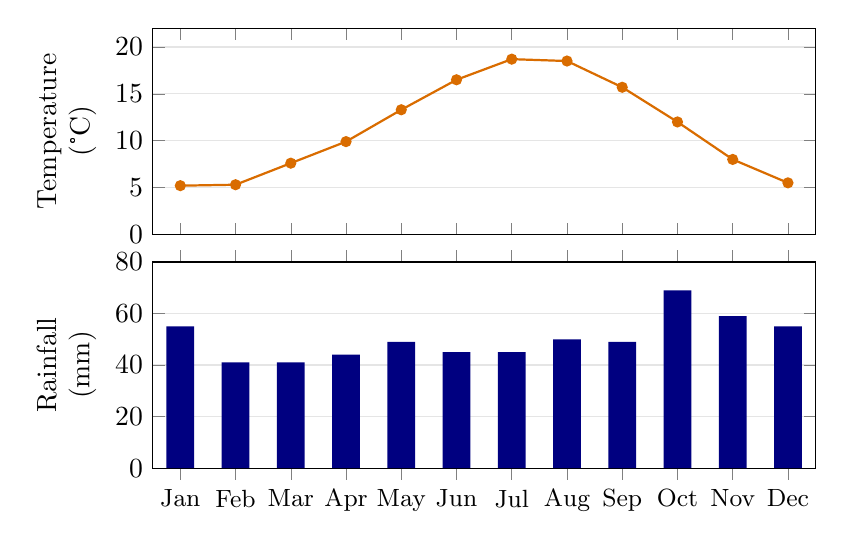
\begin{tikzpicture}
  \begin{groupplot}[
    group style={group size=1 by 2, vertical sep=0.35cm, xticklabels at=edge bottom},
    width=10cm, height=4.2cm, xmin=0.5, xmax=12.5, xtick={1,...,12},
    xticklabels={Jan, Feb, Mar, Apr, May, Jun, Jul, Aug, Sep, Oct, Nov, Dec},
    ymajorgrids, grid style={gray!20}, ylabel style={align=center}, xticklabel style={font=\small},
  ]
    \nextgroupplot[ylabel={Temperature\\(\textdegree C)}, ymin=0, ymax=22]
      \addplot[thick, orange!85!black, mark=*, mark size=1.6pt] coordinates {
        (1,5.2) (2,5.3) (3,7.6) (4,9.9) (5,13.3) (6,16.5) (7,18.7) (8,18.5) (9,15.7) (10,12.0) (11,8.0) (12,5.5)};
    \nextgroupplot[ylabel={Rainfall\\(mm)}, ymin=0, ymax=80, ybar, bar width=10pt]
      \addplot[fill=blue!50!black, draw=none] coordinates {
        (1,55) (2,41) (3,41) (4,44) (5,49) (6,45) (7,45) (8,50) (9,49) (10,69) (11,59) (12,55)};
  \end{groupplot}
\end{tikzpicture}
